\chapter{Optical Music Recognition}
\label{chap:OMR}

TODO: definition of OMR

% what is OMR (definition)

problems with I/O


\section{Approaches to OMR}

TODO: general talk about OMR datasets and that we show only related ones here

approaches to omr
    traditional pipeline
    shift to DL
    four stage pipeline
    end-to-end pipeline
        are a black box    
        limited to monophonic
    interactive systems


\section{Datasets}
\label{sec:Datasets}

When performing experiments, we will use these three datasets:

\begin{itemize}
    \item CVC-MUSCIMA (\cite{CvcMuscima})
    \item MUSCIMA++ (\cite{MuscimaPP})
    \item DeepScores v2 (\cite{DeepScores})
\end{itemize}

These are the only datasets in the OMR field that contain semantic segmentation labels (for Common Western Music Notation). A comprehensive list of available OMR datasets is maintained by Alexander Pacha on his GitHub page\footnote{\url{https://apacha.github.io/OMR-Datasets/}}.


\subsection{CVC-MUSCIMA}

This dataset was introduced in the article \emph{CVC-MUSCIMA: A ground truth of handwritten music score images for writer identification and staff removal} (\cite{CvcMuscima}). It contains 1000 pages of handwritten music, created by having 50 writers transcribe 20 unique music pages. It was designed for the tasks of staff removal and writer identification. It is also the only handwritten music dataset, consisting of entire music pages -- all other handwritten datasets contain only individual symbols. This makes it very important for research focusing on symbol detection.

\begin{figure}[ht]
    \centering
    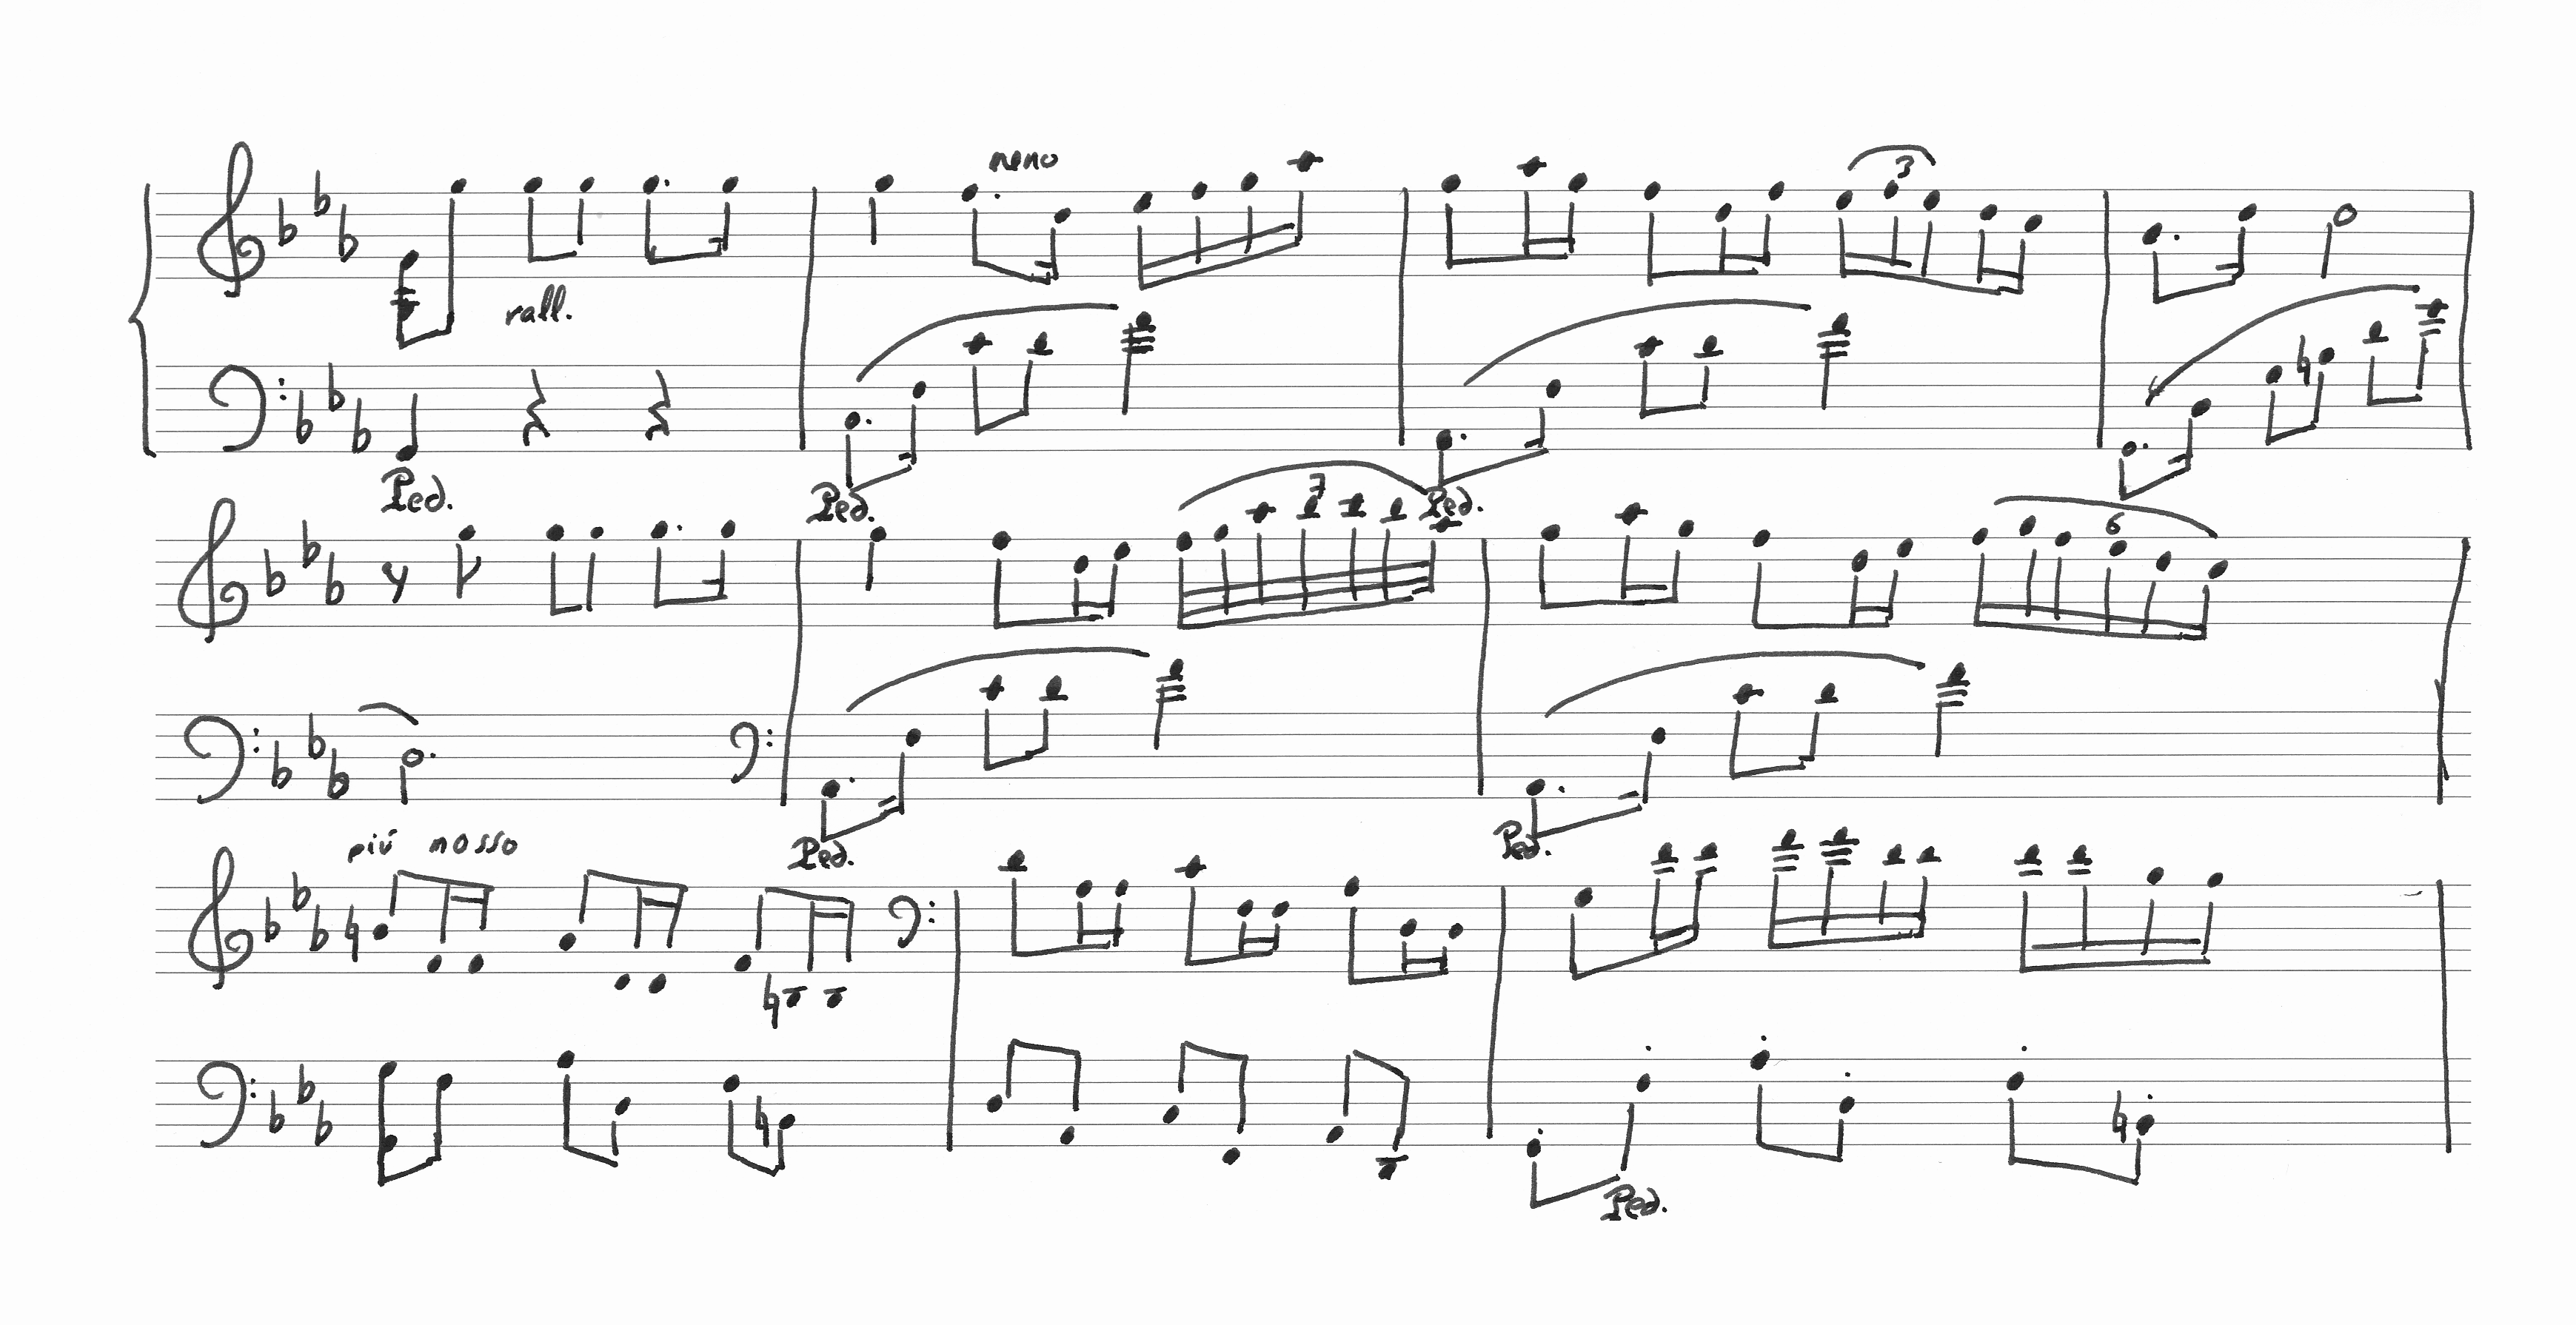
\includegraphics[width=140mm]{../img/cvc-muscima.png}
    \caption{One page from the CVC-MUSCIMA dataset. The image is taken from the website \url{http://www.cvc.uab.es/cvcmuscima/index_database.html}}
    \label{fig:CvcMuscima}
\end{figure}

Since the dataset does not contain segmentation labels, we will use it primarily as a source of unlabeled training data.


\subsection{MUSCIMA++}

MUSCIMA++ was created by Jan Hajič jr. and Pavel Pecina as a general-purpouse OMR dataset. It was introduced in the article \emph{In Search of a Dataset for Handwritten Optical Music Recognition: Introducing MUSCIMA++} (\cite{MuscimaPP}). The dataset builds on top of the CVC-MUSCIMA dataset, providing rich annotations for 140 selected pages. The annotation scheme was designed to be sufficiently low-level for tasks such as object detection (bounding boxes, symbol classes, segmentation masks), while also having relationship data in the form of an oriented graph, that lets a user extract semantic information about the music. Dataset authors call this annotation scheme the \emph{Music Notation Graph} (MuNG).

\begin{figure}[ht]
    \centering
    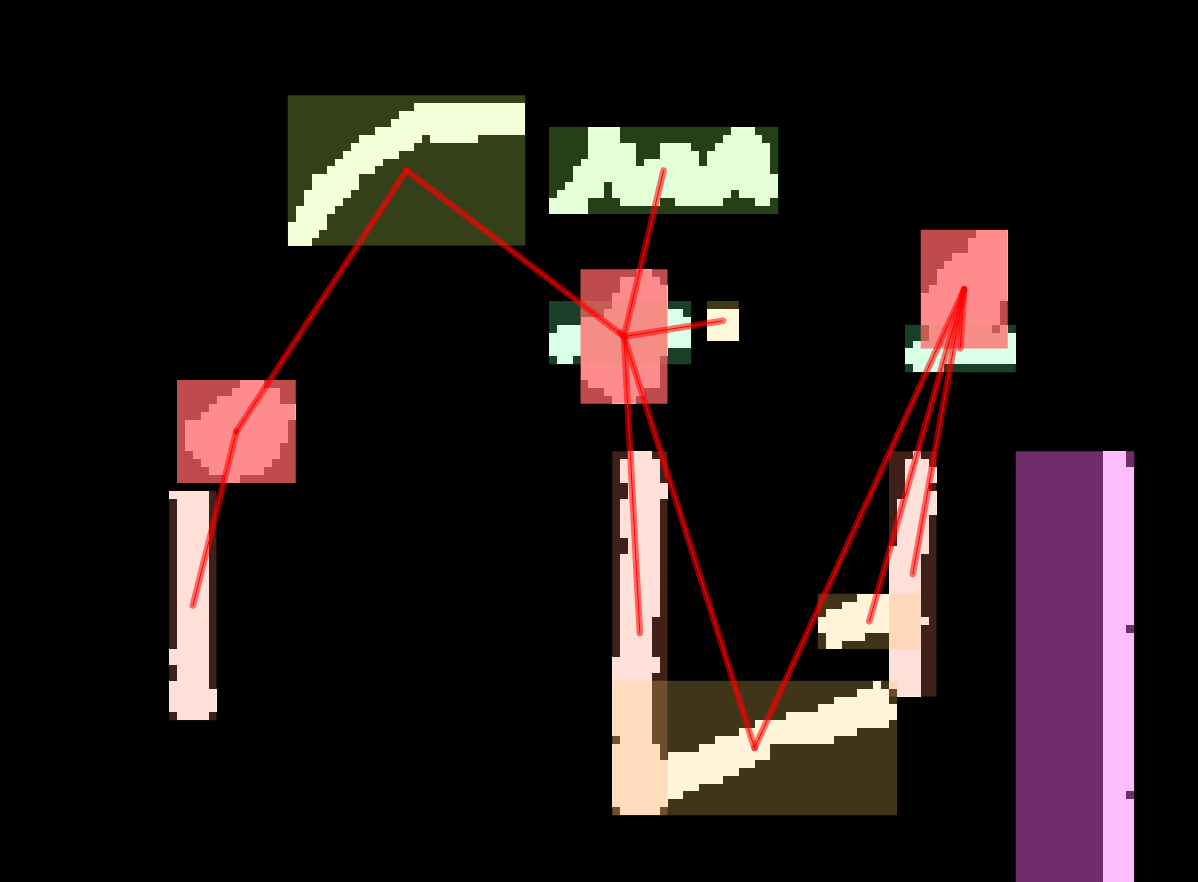
\includegraphics[width=100mm]{../img/muscima-pp.png}
    \caption{Annotations present in the MUSCIMA++ dataset (bounding boxes, segmentation masks and the notation graph). The image is taken from \cite{MuscimaPP}}
    \label{fig:MuscimaPP}
\end{figure}

The dataset was updated in 2019, fixing bugs and modifying class names to be aligned with the SMuFL\footnote{\url{https://www.smufl.org/}} standard. A similar update was also performed on the DeepScores dataset (\cite{DeepScores}), making it easier to use both datasets simultaneously. The latest dataset description and accompanying tools can be found on the GitHub page\footnote{\url{https://github.com/OMR-Research/muscima-pp}} of the OMR Research group\footnote{\url{https://omr-research.net/}}.

We will use this dataset as a source of labeled data for semantic segmentation.


\subsection{DeepScores}

The version 2 of this dataset was introduced in the article \emph{The DeepScoresV2 Dataset and Benchmark for Music Object Detection} (\cite{DeepScores}). The dataset contains entire pages of printed music, with annotations best suited for object detection, semantic segmentation and object classification. It was created from MusicXML documents taken from the MuseScore\footnote{\url{https://musescore.com/sheetmusic}} website and engraved using the LilyPond\footnote{\url{https://lilypond.org/}} tool. The dataset contains 255,386 pages of music, but also provides a dense and diverse subset, having only 1,714 pages. The version 2 also introduced a MUSCIMA++ compatibility mode, making it easier for the two datasets to be used simultaneously.

\begin{figure}[ht]
    \centering
    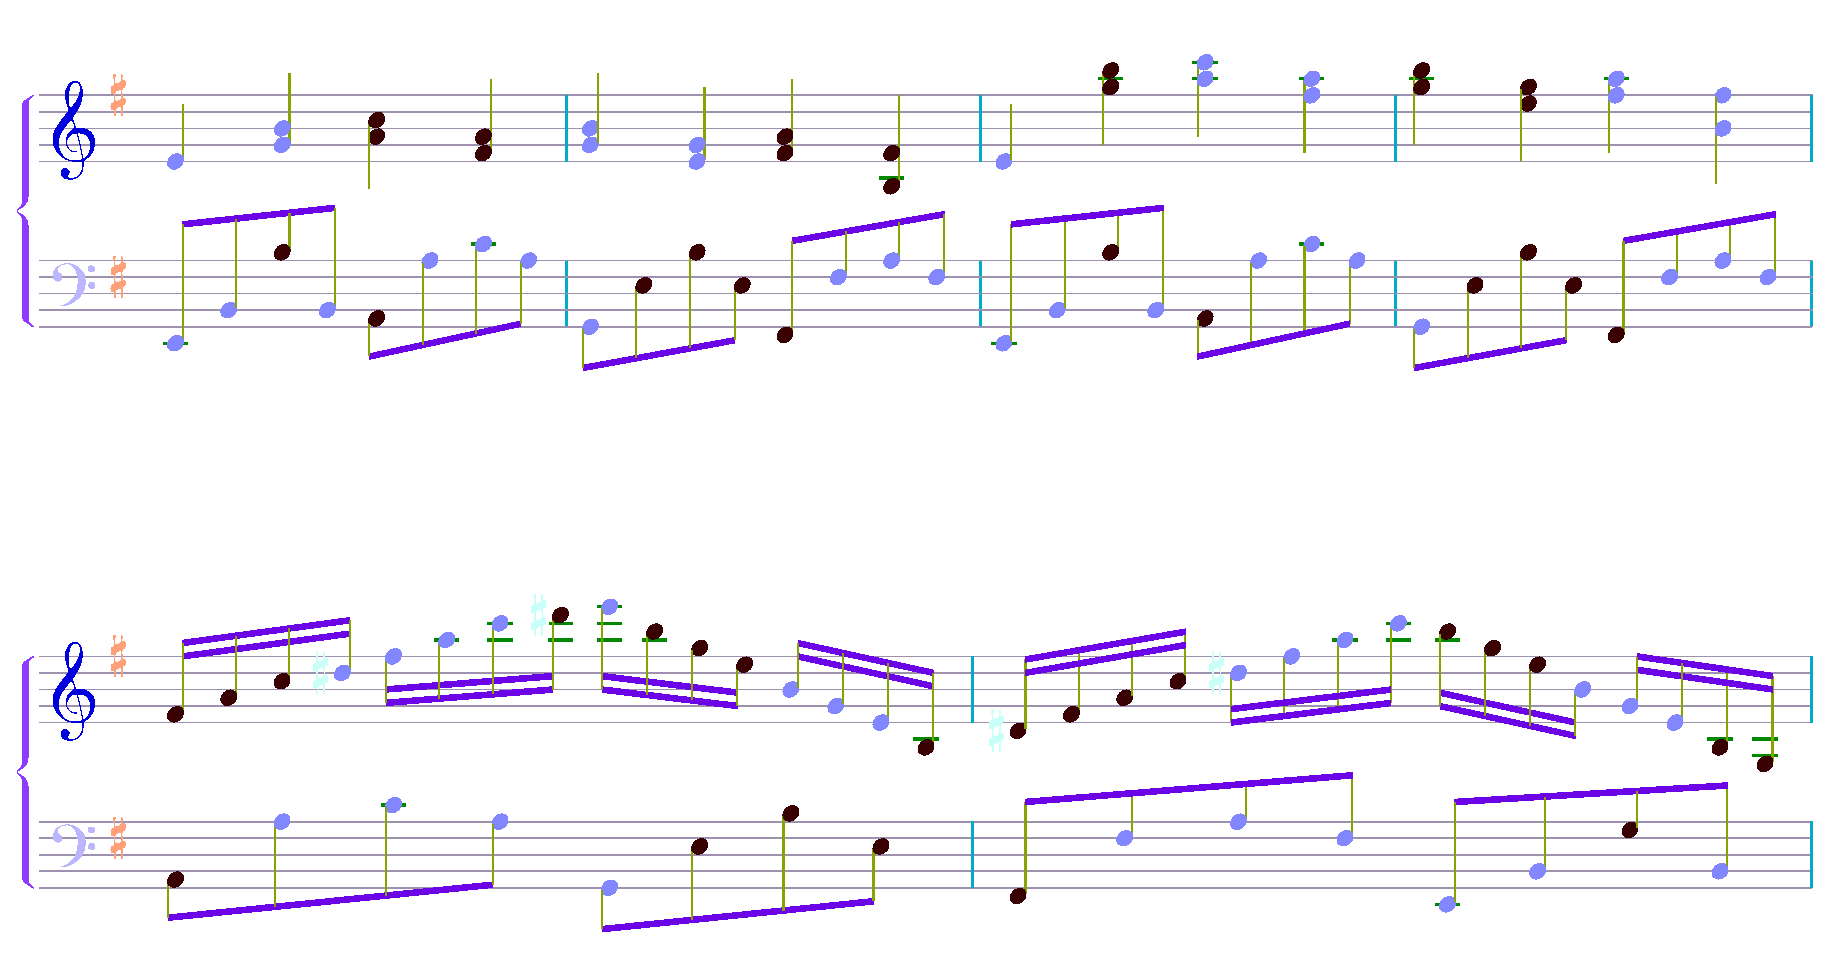
\includegraphics[width=140mm]{../img/deepscores.png}
    \caption{An example of semantic segmentation labels from the DeepScores v2 dataset. The dataset is very large, but digitally engraved.}
    \label{fig:DeepScoresV2}
\end{figure}

We will use this dataset as a source of labeled data for semantic segmentation.
